\documentclass[11pt]{oblivoir}
\usepackage{kotex}
\usepackage{graphicx} 
\usepackage{fullpage}
\usepackage{siunitx}
\usepackage[ruled,vlined]{algorithm2e}
\usepackage{hyperref}
\usepackage[nameinlink]{cleveref}
\usepackage{listings}
\usepackage{color}
\usepackage{caption}
\usepackage{indentfirst}
\usepackage{subcaption}
\usepackage{tikz-cd}

\definecolor{dkgreen}{rgb}{0,0.6,0}
\definecolor{gray}{rgb}{0.5,0.5,0.5}
\definecolor{mauve}{rgb}{0.58,0,0.82}

\lstset{frame=tb,
  language=C++,
  aboveskip=3mm,
  belowskip=3mm,
  showstringspaces=false,
  columns=flexible,
  basicstyle={\small\ttfamily},
  numbers=none,
  numberstyle=\tiny\color{gray},
  keywordstyle=\color{blue},
  commentstyle=\color{dkgreen},
  stringstyle=\color{mauve},
  breaklines=true,
  breakatwhitespace=true,
  tabsize=3
}

\crefname{figure}{그림}{그림}
\crefname{equation}{식}{식}
\crefname{table}{표}{표}
\crefname{listing}{목록}{목록}
\crefname{section}{절}{절}
\crefname{algorithm}{알고리즘}{알고리즘}

\title{AR 당구}
\author{강승우 \\ 한국기술교육대학교 전자공학과}
\date{2020.10}

\begin{document}
\maketitle

\setlength{\parindent}{0.3cm}


\begin{abstract}

        당구는 재미있는 실내 스포츠이지만, 요즘처럼 오락거리가 많은 시대에 초심자가 발을 붙이기에는 다소 진입장벽이 높다. AR 당구는 입문자들이 당구의 높은 진입장벽을 손쉽게 극복하는 데 도움을 줄 수 있도록 기획되었다. 몰입도 높은 VR HMD
        \footnote{Head Mounted Display의 약자; VR 헤드셋과 같이 머리에 장착하여 사용자의 시야 전체를 채우는 형태의 장착형 디스플레이 기기를 일컬음}
        상에서 당구공이 득점 가능한 최적의 경로 및 사용자가 취한 큐의 각도에 대한 피드백을 시각화하고, 여러 시청각 효과를 통한 오락 요소를 도입하여 입문자의 흥미 유발과 당구에 대한 감각 습득을 돕는다.

        AR 당구의 구현은 (1) 영상 처리를 통한 당구대, 당구공, 큐의 3D Pose 획득 (2) 득점 경로를 계산하기 위한 물리 시뮬레이션 구현 (3) 오브젝트의 3D 포즈 및 계산된 득점 경로 등에 대한 시각화의 세 요소를 통해 이루어진다.

        (Abstract 내 최종 구현 내용은 추후 기술)
\end{abstract}

\newpage




\section{영상 처리}
\subsection{개요}

당구공과 당구대 등 현실 세계의 물체 위에 증강현실 이펙트를 뿌려주기 전에 먼저 물체의 게임 엔진 상에서의 월드 좌표(이하 월드 좌표)를 획득해야 한다. 이는 카메라 파라미터를 통해 2D 이미지 상에서 각 오브젝트의 카메라에 대한 상대 좌표를 획득하고, 카메라의 월드 변환 행렬을 적용하는 일련의 과정으로 이루어진다.

다음은 당구대, 당구공, 큐 각각을 2D 이미지 상에서 인식하고, 3D 포즈를 추정하는 과정이다.

\subsection{당구대 인식}
\label{section;imgproc;table}
\begin{figure}[ht]
        \begin{center}
                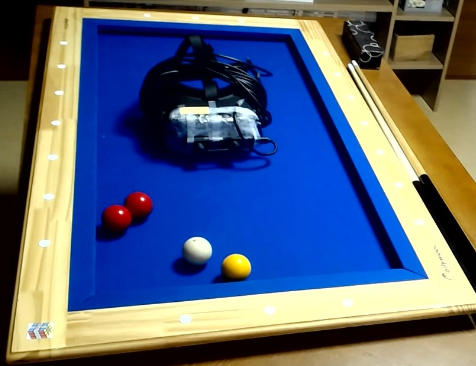
\includegraphics[width=8cm, height=8cm, keepaspectratio]{img/billiards-table.png}
        \end{center}
        \caption[Caption for LOF]{당구대 세트, VR HMD 및 HMD에 장착된 스테레오 카메라\footnotemark}
        \label{fig;pool-table}
\end{figure}

\footnotetext{휴대성, 작업의 용이성, 경제성 등을 고려하여 작은 크기의 미니 당구 세트를 활용하였다.}

\cref{fig;pool-table}의 당구대를 보면 당구대 펠트의 진한 파란색이 주변과 매우 뚜렷하게 구분되는 것을 볼 수 있다. 이 이미지를 HSV 색공간으로 표현하면(\cref{fig;pool-table-hs}) Hue와 Saturation 영역에서 당구대의 영역이 뚜렷하게 식별되며, 이를 Hue 175$\sim$20\si{\degree}, Saturation 160$\sim$255, Value 0$\sim$255의 범위로 필터링\footnote{cv::inRange 함수}하면 \cref{fig;pool-table-edge}의 결과를 얻는다.

\begin{figure}[ht]
        \begin{center}
                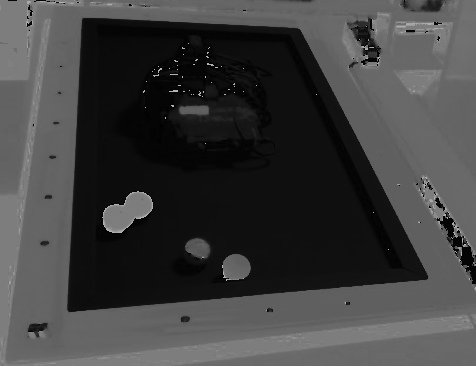
\includegraphics[width=5cm, height=5cm, keepaspectratio]{img/billiards-table-h-shift.png}
                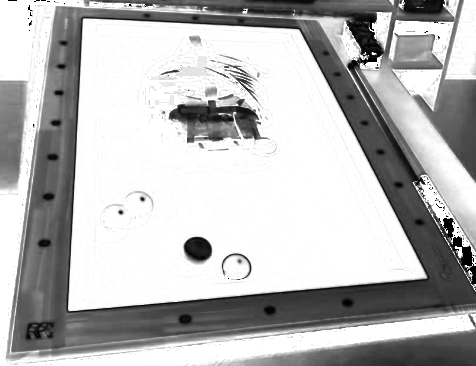
\includegraphics[width=5cm, height=5cm, keepaspectratio]{img/billiards-table-s.png}
                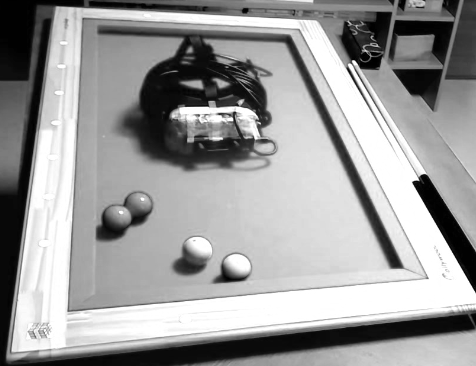
\includegraphics[width=5cm, height=5cm, keepaspectratio]{img/billiards-table-v.png}
        \end{center}
        \caption[Caption for LOF]{\cref{fig;pool-table}의 HSV 색공간 변환 이미지. 왼쪽부터 H\footnotemark, S, V}
        \label{fig;pool-table-hs}
\end{figure}

\cref{fig;pool-table-edge}의 우측 에지 이미지는 필터링 결과를 1회 침식한 후 빼서 에지를 검출한 결과이다.

\begin{figure}[ht]
        \begin{center}
                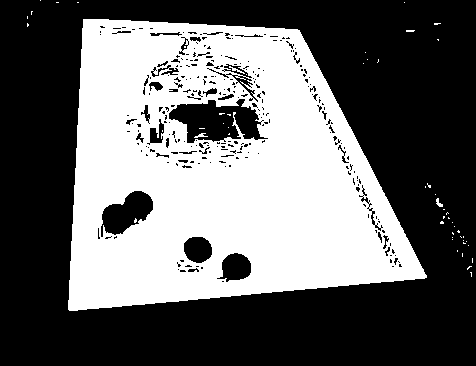
\includegraphics[width=5cm, height=5cm, keepaspectratio]{img/billiards-table-filter.png}
                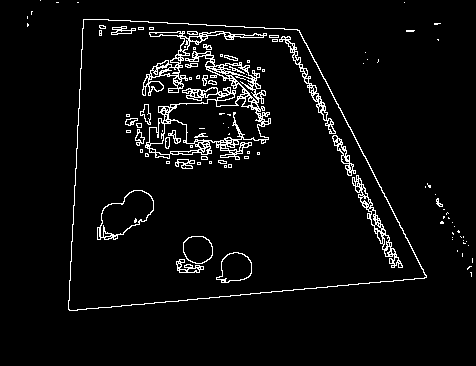
\includegraphics[width=5cm, height=5cm, keepaspectratio]{img/billiards-table-edge.png}
                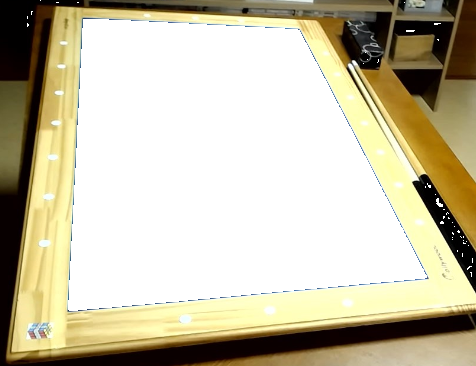
\includegraphics[width=5cm, height=5cm, keepaspectratio]{img/billiards-table-contours.png}
        \end{center}
        \caption{왼쪽부터 필터링 적용, 침식 연산을 통한 경계선 검출, findContours 적용 결과}
        \label{fig;pool-table-edge}
\end{figure}

\footnotetext{이 때, Hue 이미지는 파란색이 0도와 180도에 걸쳐 있어서, 5\si{\degree} 우측으로 시프트.}

\cref{fig;pool-table-edge}의 경계선은 당구대의 음영에 의해 다소 지저분하게 보이지만, 이 단계의 목적이 되는 테이블의 경계선은 뚜렷하게 식별된다. 이 때 contour 탐색 함수\footnote{cv::findContours 함수}를 활용해 테이블 영역의 각 정점을 추출해낼 수 있다.

이 때 단순히 색상이 비슷한 물체를 당구대 영역으로 잘못 탐지하는 것을 막기 위해 간단한 필터링 알고리즘을 적용한다. 일차적으로 컨투어 영역의 픽셀 크기가 일정 값 이하인 모든 컨투어를 버리고, contour point approximation과 convex hull 알고리즘
\footnote{cv::approxPolyDP, cv::convexHull 함수}
을 적용해 모든 컨투어를 최대한 단순화한다.

단순화된 컨투어 중 면적이 가장 크고, 정점의 개수가 4개 이상인 컨투어가 당구대의 후보가 된다.
\footnote{이 때 approxPolyDP와 convexHull 함수의 적용으로, 당구대 영역을 침범하는 외부 물체에 대해서도 어느 정도 tolerance를 갖게 된다.}

후보의 정점 개수가 정확히 4개인 경우 Perspective N-Point 알고리즘을 적용해 정확하게 당구대의 포즈를 계산해낼 수 있다. 단, 알고리즘이 정확하게 당구대의 포즈를 추정해내기 위해선 먼저 화면 상의 각 점의 순서가 반드시 모델 좌표계의 당구대의 순서와 일치해야 한다.

\cref{fig;pool-table-invalid-index}에서와 같이 인덱스가 잘못 지정된 경우를 해소하기 위해, Stereo camera로부터 얻어진 깊이 이미지에서 당구대 후보의 네 점에 대한 깊이 값을 획득하고, 이를 3D 좌표로 변환하여 각 변의 추정 길이를 계산한다.
\footnote{깊이 이미지로 얻어진 각 픽셀의 3D 좌표는 값이 거의 10 cm 수준에서 진동하여 신뢰하기 어려우므로, 깊이 이미지는 이 단계에서만 활용하고 이후에는 사용하지 않는다.}

\begin{figure}[ht]
        \begin{center}
                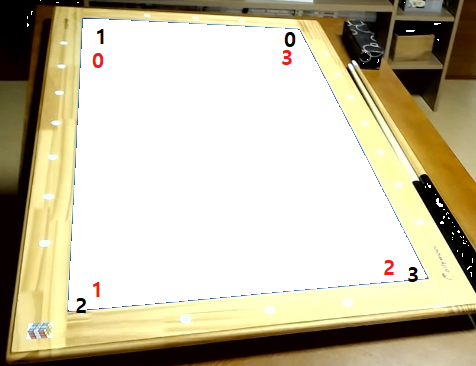
\includegraphics[width=8cm, height=5cm, keepaspectratio]{img/billiards-table-indexes.png}
        \end{center}
        \caption{인덱스 순서는 위와 같이 어긋날 수 있다.}
        \label{fig;pool-table-invalid-index}
\end{figure}

추정 3D 포인트를 두 개의 인덱스씩 순회하여 짧은 변이 먼저 나타난다면 그대로 두고, 긴 변이 먼저 나타나면 컨투어의 정점 목록을 하나씩 회전시키는 식이다.

정렬된 컨투어의 정점 목록과 모델 공간의 테이블 정점 목록을 인자로 PNP 알고리즘
\footnote{cv::solvePnP 함수, iterative method 적용}
을 적용하면 카메라에 대한 테이블의 relative position과 rotation을 획득할 수 있다. 이를 카메라 월드 트랜스폼으로 변환해주면 테이블의 월드 위치 및 회전을 획득할 수 있다.

단, 이 경우 테이블의 회전 수치는 180\si{\degree} 회전된 값이 반환될 수 있는데, 이 경우 마지막으로 보고된 테이블의 월드 로테이션과 비교하여 각도의 차이가 175\si{\degree} 이상인 경우 단순히 180\si{\degree}를 제하는 것으로 보정한다.

\subsubsection{테이블의 일부만 시야에 들어온 경우}

테이블의 일부만이 시야 내에 있어 컨투어의 정점 개수가 5개 이상 검출되는 경우에는 PNP 알고리즘을 적용할 정확한 정점의 위치를 파악하기 어렵다. 하지만, 적어도 두 개 이상의 코너가 시야 내에 잡혔다면 테이블의 포즈를 추정하는 것이 가능하다.

\begin{figure}[h]
        \centering
        \begin{subfigure}{0.4\textwidth}
                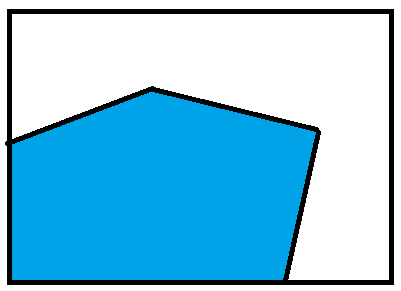
\includegraphics[width=\textwidth]{img/partial-table-valid-case.png}
                \caption{위치를 추정할 수 있음}
        \end{subfigure}
        \centering
        \begin{subfigure}{0.4\textwidth}
                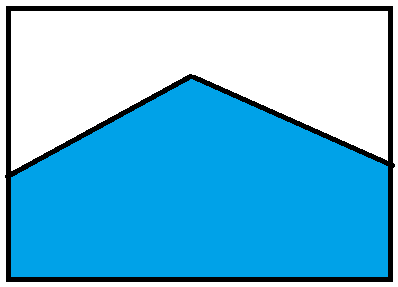
\includegraphics[width=\textwidth]{img/partial-table-invalid-case.png}
                \caption{위치 추정이 불가}
        \end{subfigure}
        \caption{테이블의 일부분만 시야에 들어오는 경우}
\end{figure}

임의의 position과 rotation으로 테이블의 모델을 화면에 투영하고, 투영된 컨투어 목록과 검출된 컨투어 목록 사이의 오차를 계산하여 반복적으로 오차를 줄여나가는 방법이다.

그러나 단순히 컨투어 목록을 OpenCV가 제공하는 projection method
\footnote{cv::projectPoints}
를 활용하면 일부 정점은 단순히 화면 밖으로 투영되고, \cref{fig;invalid-sight-projection}에서와 같이 화면의 경계선에 걸쳐 있는 점들과의 오차를 제대로 계산할 수 없다. 따라서 모델 정점들을 화면에 투사하기 전, 먼저 시야 범위를 구성하는 네 개의 평면에 맞춰 범위를 벗어나는 정점들에 대해 절단을 수행한다.

\begin{figure}[h]
        \centering
        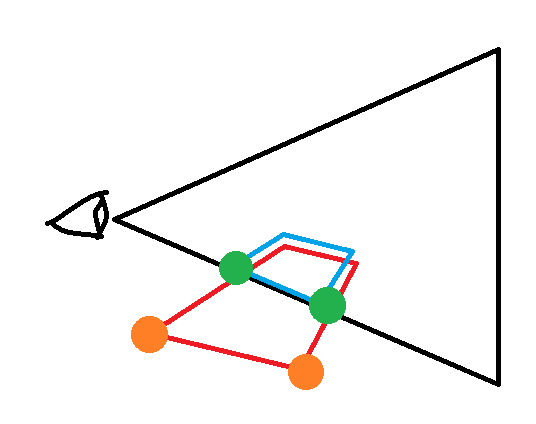
\includegraphics[width=7cm]{img/sight-invalid-culling.png}
        \caption{모델 정점을 그대로 화면에 투사할 시 일부 정점이 화면에서 이탈한다}
        \label{fig;invalid-sight-projection}
\end{figure}

위 과정을 거쳐 추정 위치 및 회전으로 투사된 정점 목록을 검출된 정점과 비교해 오차를 계산한다. 이 때  투사된 정점 목록의 인덱스를 시계 방향으로 한 번씩 회전시키며, 정점 사이의 거리(오차)의 합 $\sum_{n=0}^{N}|\vec{P}_{pn} - \vec{P}_{sn}|$이 최소치가 되는 트랜스폼을 선택한다.

이후 위와 마찬가지로 카메라에 대한 테이블의 상대 포즈를 월드 좌표로 변환한다.



\subsection{당구공 인식}

\begin{figure}[ht]
        \centering
        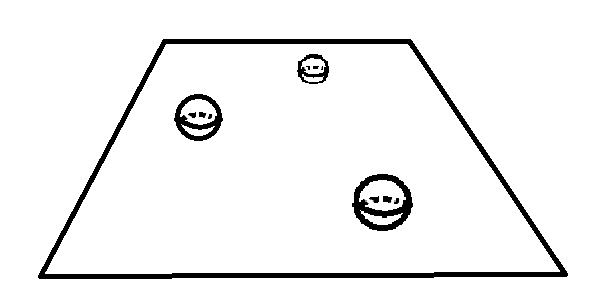
\includegraphics[width=8cm]{img/ball-recognition-introduce.png}
        \caption{당구공의 중점은 항상 한 평면상에 존재한다}
        \label{fig;ball-recognition-intro}
\end{figure}

당구공은 완전한 구의 형태이며, 따라서 카메라에서 2D 이미지 상 원형의 중점으로 광선(a)을 투사하면 반드시 구의 중점을 지나게 된다. 또, 구의 중점은 반드시 당구대 표면에서 일정한 거리로 떨어진 평면(b) 상에 존재한다.

이 과정은 \cref{fig;ball-recognition-howto}에 잘 나와있다.

\begin{figure}[ht]
        \centering
        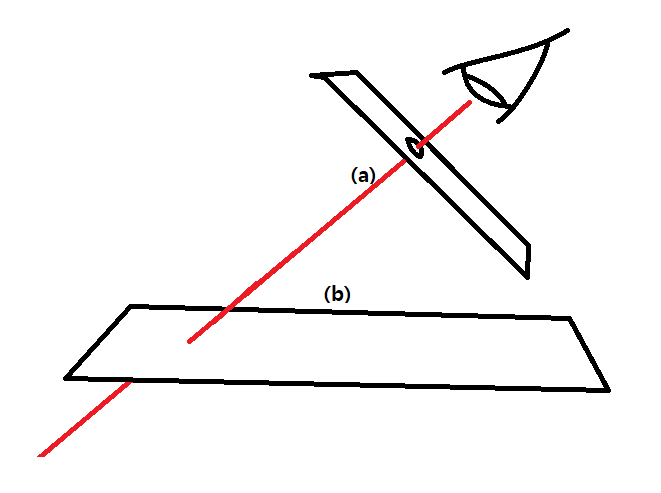
\includegraphics[width=8cm]{img/ball-recognition-howto.png}
        \caption{(b)는 당구공의 중점이 존재할 수 있는 평면이다}
        \label{fig;ball-recognition-howto}
\end{figure}

이미 위에서 테이블의 3D 포즈를 계산하였다. 이렇게 계산된 포즈는 테이블의 바깥쪽 쿠션 높이를 기준으로 한 평면이므로(\cref{fig;cushion-height-example}의 A), 평면 (b)는 테이블 평면을 노멀 반대 방향으로 약간 오프셋하여 손쉽게 계산할 수 있다.

\begin{figure}[ht]
        \centering
        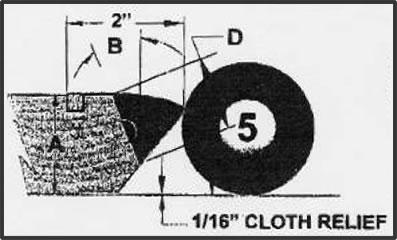
\includegraphics[width=8cm]{img/cushion-height-example.png}
        \caption[Caption for LOF]{당구대 쿠션 높이 예시\footnotemark}
        \label{fig;cushion-height-example}
\end{figure}
\footnotetext{이미지 출처: https://www.pooltablefeltcloth.com/cushion-height-guide-for-k-66-k-55.html}

다음으로 필요한 것은 각 공의 중점을 찾아내는 것이다. 탑-다운으로 이미지를 촬영해 이미지 상에서 공의 크기가 균일하고 공 사이에 폐색$_\text{occlusion}$이 발생하지 않는 일반적인 당구 보조 프로그램과 달리, AR 당구는 사용자 시점에서 영상 인식을 수행해야 하기 때문에 거리에 따라 구체의 이미지 상 반지름이 다르고, 폐색 또한 발생할 수 있다.

\begin{figure}
        \centering
        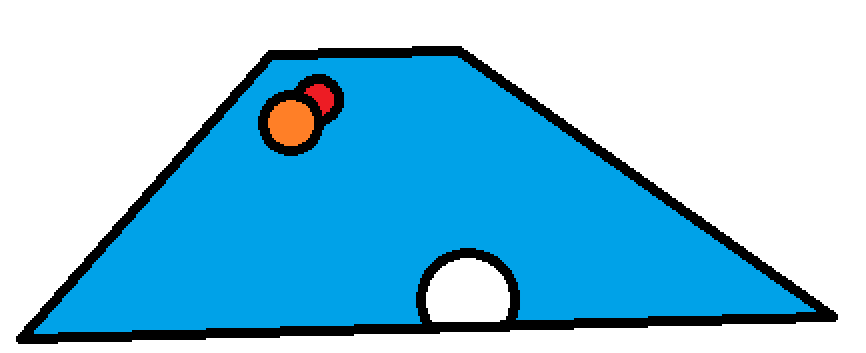
\includegraphics[width=8cm]{img/billiards-ar-view.png}
        \caption{AR 당구의 당구공 인식은 더 많은 요인을 고려해야 한다}
\end{figure}
카메라로부터의 거리에 따라 변화하는 공 원형의 반지름에 대응하기 위해 공을 검출하기 위한 커널의 크기를 매 평가시마다 동적으로 조절한다. 이 과정은 \cref{algo;kernel-radius}에 서술되어 있듯, 임의의 2D 점에 대한 먼 3D 점을 구하고, 카메라 원점 $(0, 0, 0)$과 해당 점 사이에 광선을 투사해 평면 (b)와 만나는 지점의 z 값을 찾음으로써 이루어진다. 

\begin{algorithm}
        \caption{Estimate ball radius scale of given pixel coordinate}
        \label{algo;kernel-radius}
        \SetAlgoLined
        $\vec{P}_{ball} (u, v) \gets$ [Input] 2D point of estimated circle center \\
        $\vec{P}_{ray} (x, y, z) \gets$ $\vec{P}_{ball}$'s 3D coordinate assuming z as 10 \\
        $\vec{P}_{ball3} (x, y, z) \gets$ contact between $(0, 0, 0)$ and $\vec{P}_{ray}$ on the table plane (b) \\
        \KwResult{Evaluation kernel's radius scale is $z^{-1}$}
\end{algorithm}

\subsubsection{적합도 평가}
일반적으로, AR 당구의 사용자 시점에서 공은 다른 공에 의해 폐색될 수 있다. 즉, 많은 경우 공을 찾는 알고리즘은 오차가 적은 공보다 더 가능성이 높아 보이는 공을 찾게 된다. 이 과정을 직관적으로 수행하기 위해 각 중점 후보를 평가하는 과정에서 오차치가 아닌 적합도를 계산한다.

적합도는 오차 $\epsilon$에 대한 함수로, 적합도 $$a=\alpha^{-\epsilon^2}$$로 계산한다(\cref{fig;suitability-alpha-comparison}). 이 때 $\alpha$는 적합도의 허용치를 결정하는 계수로 여기서는 1.015로 두었다. 이 식에서 각 경우(픽셀 또는 정점의 비교, 후술)의 적합도 최대치는 오차가 0인 경우 1이다. 

\begin{figure}[ht]
        \centering
        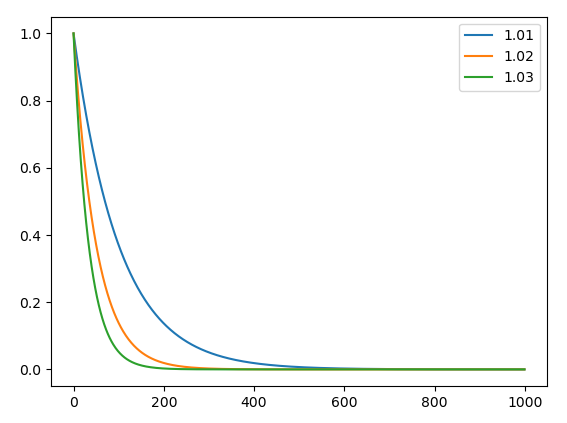
\includegraphics[width=7cm]{img/suitability-alpha-comparison.png}
        \caption{$\alpha$ 값에 따른 오차에 대한 적합도 그래프}
        \label{fig;suitability-alpha-comparison}
\end{figure}

\subsubsection{경계 적합도}
먼저 이미지의 HSV 색공간 표현에 대해 각 공 별로 필터링을 적용, 




\end{document}
